\documentclass[10pt,twocolumn,letterpaper]{article}

\usepackage{cvpr}
\usepackage{times}
\usepackage{epsfig}
\usepackage{graphicx}
\usepackage{amsmath}
\usepackage{amssymb}
\usepackage{booktabs}
\usepackage{float}
\usepackage{enumitem}

% If you comment hyperref and then uncomment it, you should delete
% egpaper.aux before re-running latex.  (Or just hit 'q' on the first latex
% run, let it finish, and you should be clear).
\usepackage[breaklinks=true,bookmarks=false]{hyperref}

\cvprfinalcopy % *** Uncomment this line for the final submission

\def\cvprPaperID{****} % *** Enter the CVPR Paper ID here
\def\httilde{\mbox{\tt\raisebox{-.5ex}{\symbol{126}}}}

% Pages are numbered in submission mode, and unnumbered in camera-ready
%\ifcvprfinal\pagestyle{empty}\fi
\setcounter{page}{1}
\begin{document}

%%%%%%%%% TITLE
\title{Timestamping Video Game Eliminations with Computer Vision}

\author{Paul Yoon\\
Stanford University\\
{\tt\small pauljy@stanford.edu}
% For a paper whose authors are all at the same institution,
% omit the following lines up until the closing ``}''.
% Additional authors and addresses can be added with ``\and'',
% just like the second author.
% To save space, use either the email address or home page, not both
\and
}

\maketitle
%\thispagestyle{empty}

%%%%%%%%% ABSTRACT
\begin{abstract}
    Recent growth in user-generated gaming video has outpaced the tools needed to sift highlights from hours-long streams. Even the simplest gaming montage still demands that creators replay footage at normal speed to locate every elimination banner, a workflow that consumes more time than the edit itself. Existing approaches to fully-automatic highlight generation rely on heavyweight action recognition models or dense temporal annotation. This paper shows that a single-class object detector, trained on only 200 frames, is sufficient to timestamp eliminations with frame-level precision. We down-sample public and self-recorded mobile game footage to 360 p and 2 fps, annotate a bounding box around the heads-up-display kill-feed banner whenever it appears, and fine-tune YOLOv8-nano on this dataset. The results demonstrate that compact detectors and minimal supervision suffice for reliable event timestamping, offering a practical foundation for lightweight editing tools.

\end{abstract}
%%%%%%%%% BODY TEXT
\section{Introduction}

Academic work on automatic highlight generation has focused on esports broadcasts, leveraging multimodal cues such as crowd audio, casters’ pitch, or real-time win-probability curves. These systems typically employ heavyweight 3D CNNs or action-recognition pipelines that require dense temporal labels and GPU-class hardware, making them impractical for creator-side use.
\cite{RINGER2022100338} \cite{10.1145/3341105.3373894}

 Moreover, reported benchmarks target desktop titles (e.g., League of Legends, CS:GO, Valorant), leaving the rapidly growing mobile-esports segment largely unexplored.

Brawl Stars illustrates this gap. Despite hosting monthly world-finals with multimillion-viewership, it has no public dataset for kill-feed or elimination events. The only openly available computer-vision resources focus on in-game entities or UI icons unrelated to timestamping. \cite{brawl-stars-detection-mcxpk_dataset}
 Consequently, content creators still scrub recordings frame-by-frame to locate each elimination.

In response, we curate the first elimination-banner\ref{fig:kill_banner} dataset for Brawl Stars and show that a single-class detector, fine-tuned on under 200 frames and run on a 360p, 2 fps video, can timestamp kills with sub-frame precision in real time on a laptop CPU. Our extremely lightweight pipeline closes the usability gap between academic highlight detection and creator workflows, and offers a reproducible benchmark for future research on mobile-game event understanding.

\begin{figure}[H]
\centering
    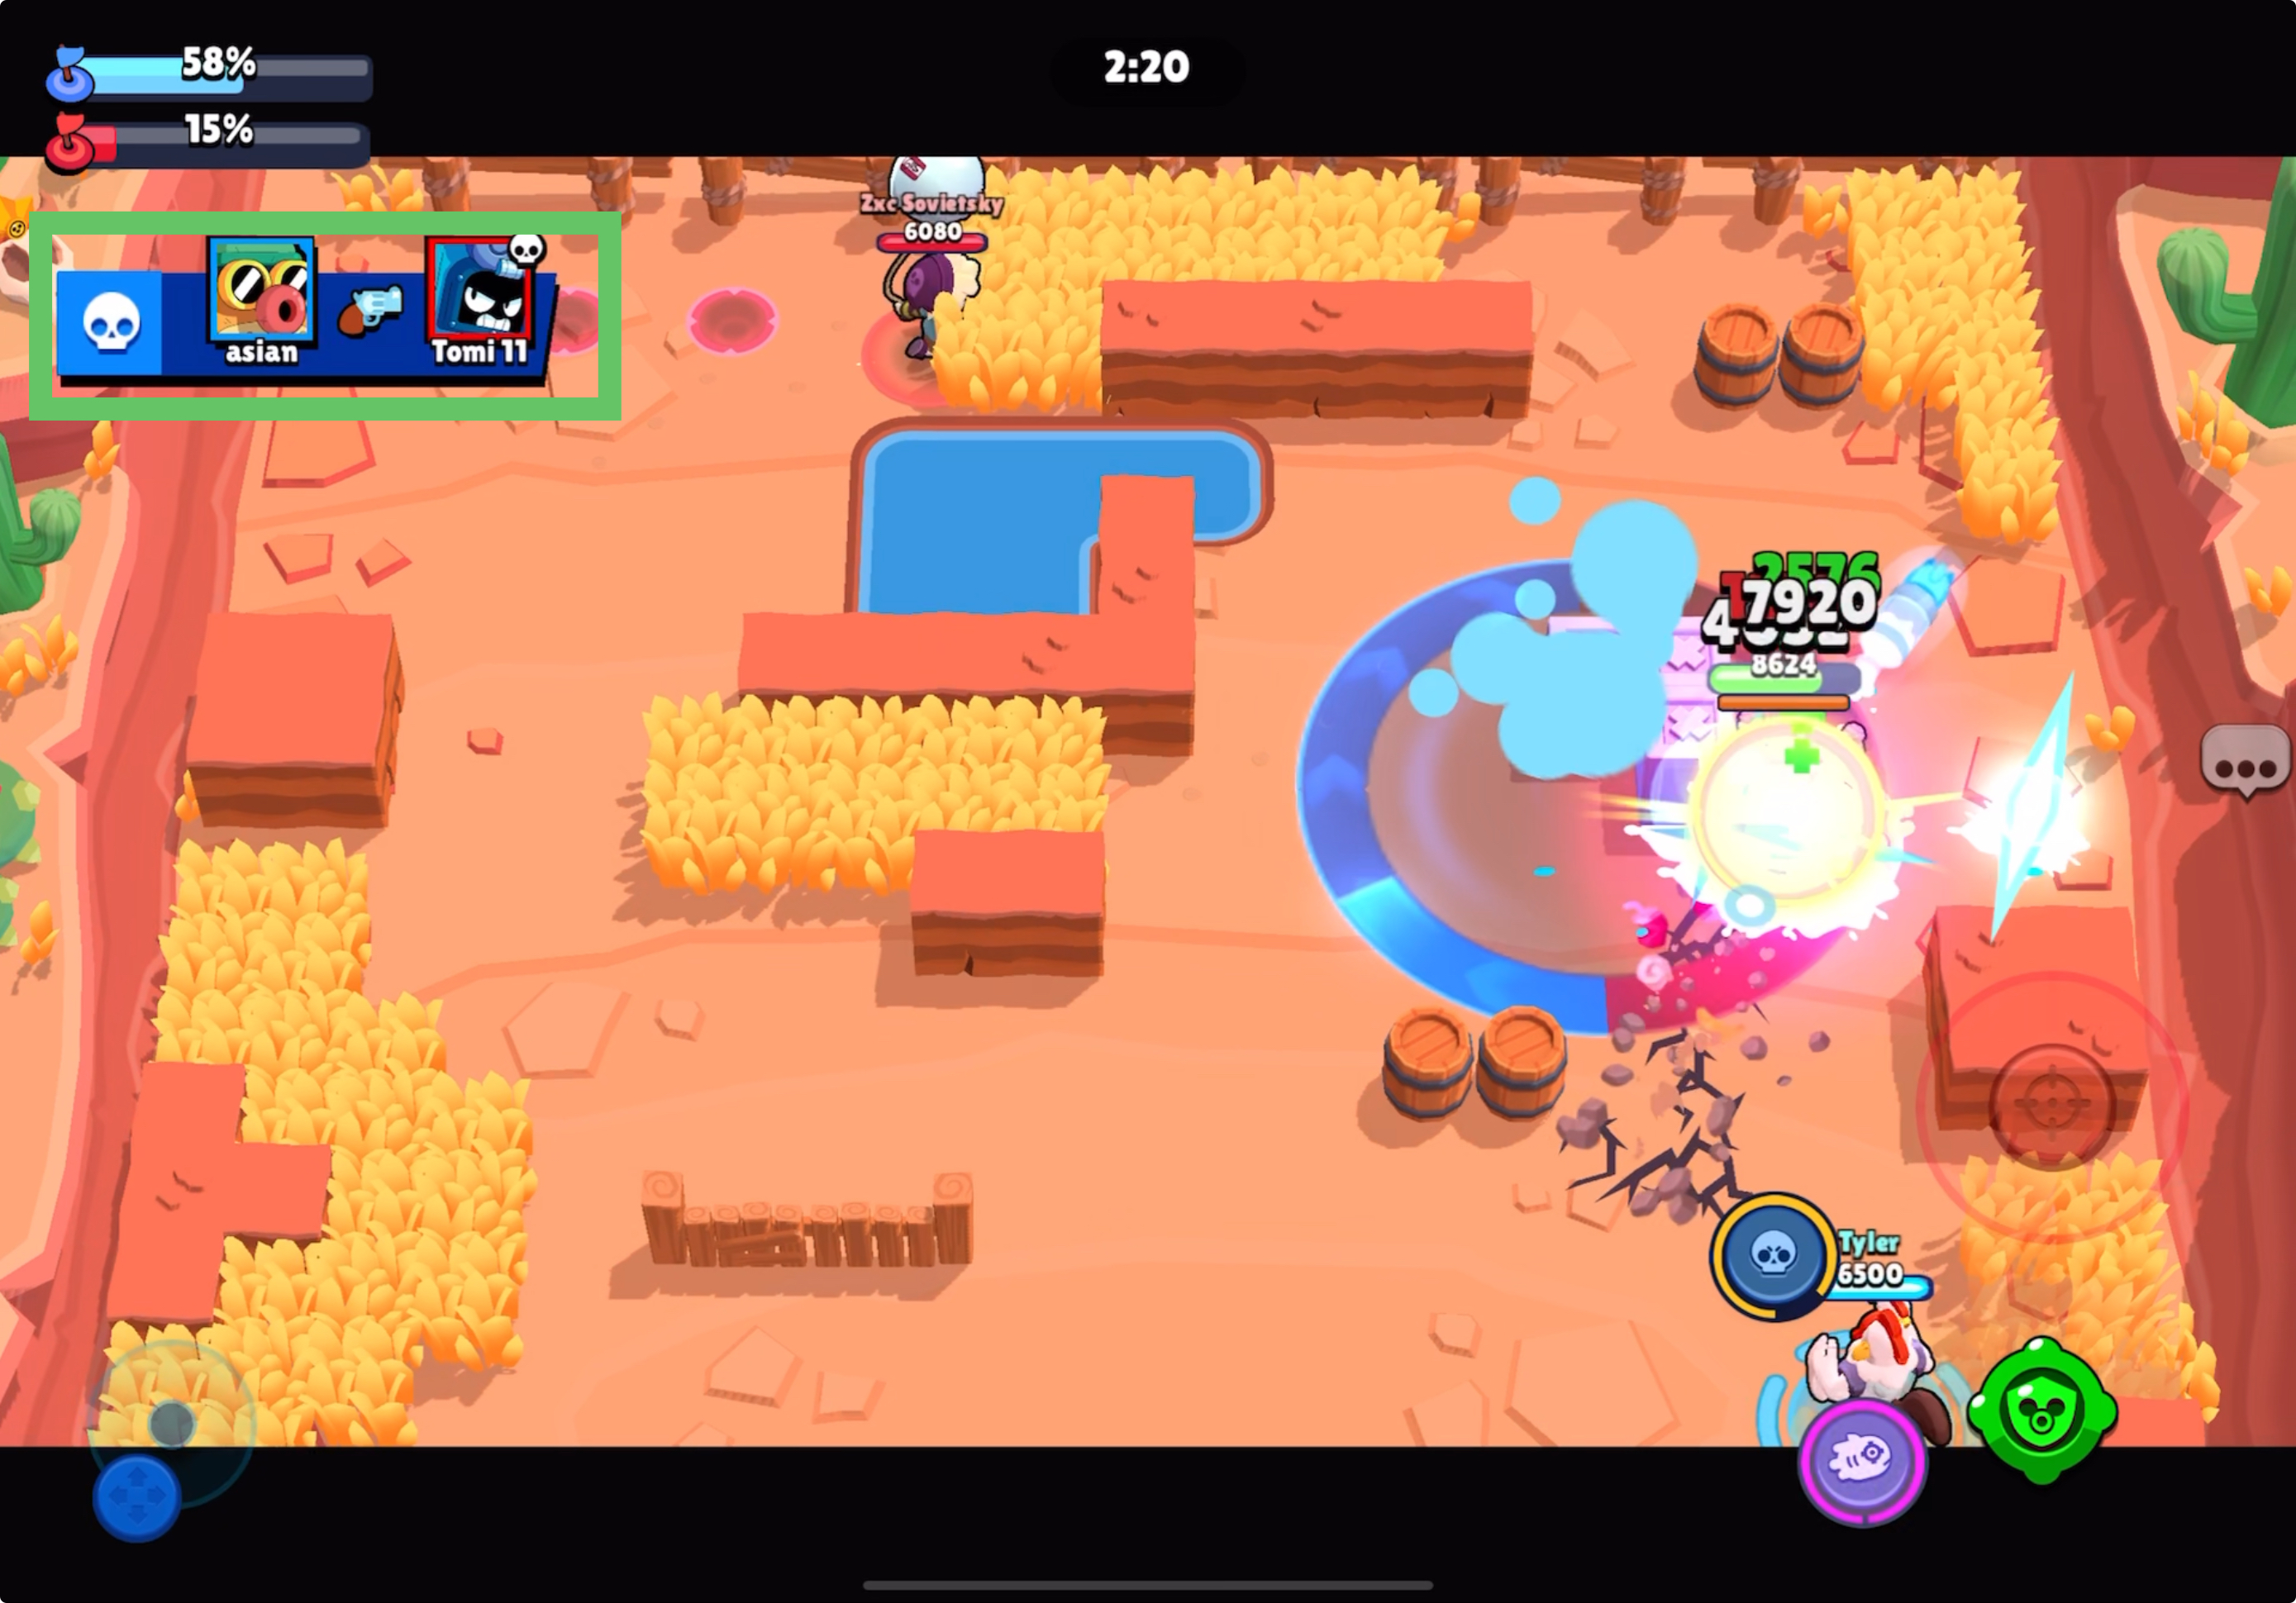
\includegraphics[scale=0.07]{brawl_stars_kill_banner.jpeg}
    \caption{a kill banner (boxed in green) appearing in \textit{Brawl Stars} gameplay}
    \label{fig:kill_banner}
\end{figure}

%-------------------------------------------------------------------------

\section{Dataset}

\subsection{Source footage}
With the lack of an official labeled kill banner dataset for \textit{Brawl Stars}, we are forced to take matters into our own hands. 
We downloaded a \textbf{14-minute}, 360 p, 30 fps video containing five ranked
\textit{Brawl Stars} matches captured on an iPad~Pro.
The footage is down-sampled offline to the working
resolution of 514\(\times\)360.

\subsection{Frame extraction}
To minimise annotation effort we extract only
two frames per second
%
\begin{equation}
    N_{\text{frames}}
      = 14\;\text{min}\;\times 60\;\frac{\text{s}}{\text{min}}
        \times 2\;\frac{\text{frames}}{\text{s}}
      \approx 1{,}650,
\end{equation}
%
using \texttt{ffmpeg}:
\begin{verbatim}
ffmpeg -i games.mp4 -vf "fps=2" /
        frames/%06d.jpg
\end{verbatim}

This is due to the fact that each kill banner persists for $\approx 1$ second after appearing. Each image is letter-boxed to 640\(\times\)640 with
black padding to preserve aspect ratio, matching YOLOv8’s default
\texttt{imgsz=640}.

\subsection{Annotation protocol}
We import the 1\,650 candidate frames into Roboflow Annotate
and draw a single bounding box around the kill-feed banner
whenever it appears.
One Hundred and Sixty Five banner images are labelled (\(n=165\));
the remaining 1\,485 frames are treated as background negatives.

\vspace{0.3em}\noindent
\textbf{Data split.}
Roboflow automatically stratifies the labelled set into
70/20/10 \% train/val/test:
%
\[
|\mathcal{D}_{\text{train}}| = 115,\;\;
|\mathcal{D}_{\text{val}}|   = 33,\;\;
|\mathcal{D}_{\text{test}}|  = 17.
\]

\subsection{Data augmentation}
We adopt YOLOv8’s built-in \emph{colour-jitter}.  
For every RGB frame \(\mathbf{x}\in[0,1]^{H\times W\times3}\) we:

\begin{enumerate}\itemsep2pt
  \item convert \(\mathbf{x}\) to \(\mathrm{HSV}\);
  \item sample
        \[
          \delta_h\sim\mathcal{U}(-30^{\circ},\,30^{\circ}),\quad
          \alpha_s,\alpha_v\sim\mathcal{U}(0.8,\,1.2);
        \]
  \item apply
        \(
          h\leftarrow(h+\delta_h)\bmod1,\;
          s\leftarrow\mathrm{clip}(\alpha_s\,s),\;
          v\leftarrow\mathrm{clip}(\alpha_v\,v)
        \);
  \item convert back to RGB.
\end{enumerate}

The three stochastic operations—hue shift,
saturation scale, brightness scale—yield  
\(\;\)one augmented replica each, so every labelled frame produces
\(1\;(\text{orig})+3=4\) training images, i.e.\ \(115\times4=460\) total.
Geometry is unchanged, so bounding-box coordinates remain valid.
The dataset is exported in Ultralytics format
(\texttt{train/images}, \texttt{train/labels}, …) referenced by
\texttt{data.yaml}.

%-------------------------------------------------------------------------

\section{Methods}
\label{sec:methods}

\subsection{Model}
We fine-tune \textbf{YOLOv8-nano} (2.5 M parameters) for a single class
\emph{kill\_banner}.
Training is invoked with:

\begin{verbatim}
yolo train model=yolov8n.pt \
     data=data.yaml \
     imgsz=640 epochs=25 batch=16 \
     freeze=10
\end{verbatim}

\noindent The model architecture is as follows:
\begin{figure}[H]
  \centering
  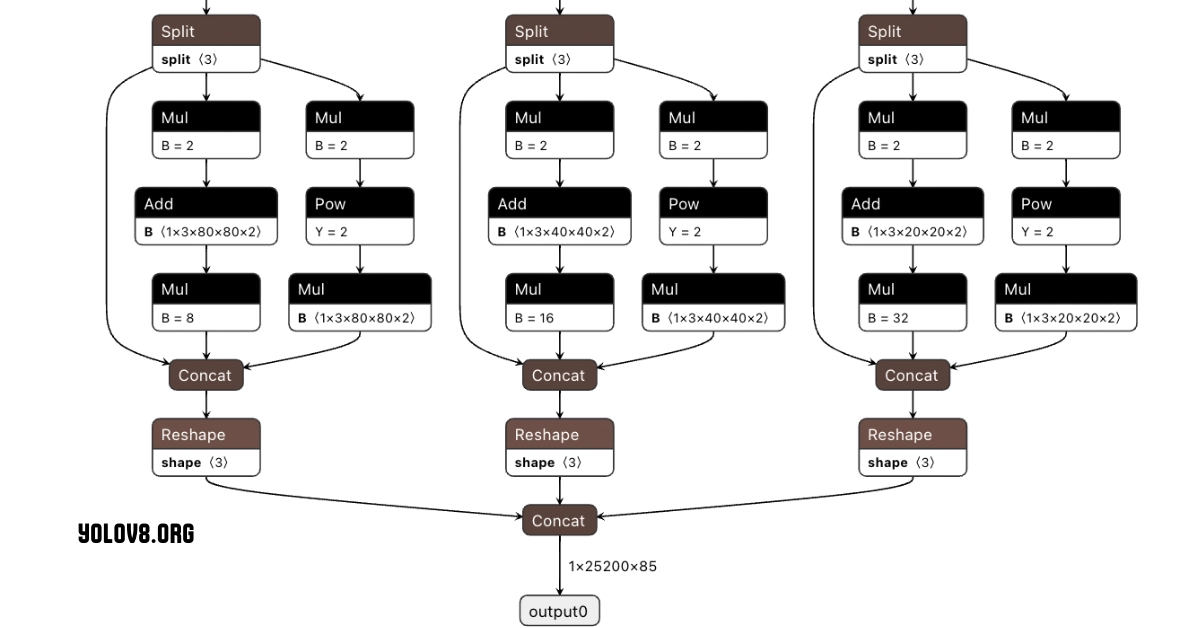
\includegraphics[width=\linewidth]{yolo-architecture.jpg}
  \caption{YOLOv8‐nano detection head.  The backbone (not shown) is a
  129-layer CSP encoder; only the three-scale head is visualised here.
  Courtesy of Ultralytics \cite{torres2025yolov8}.}
  \label{fig:yolov8-head}
\end{figure}


\noindent
\textbf{Training details.}
\begin{itemize}\itemsep2pt
  \item Optimiser: SGD, initial \(lr = 0.01\), momentum 0.937.
  \item Losses: standard YOLOv8 (objectness, box, cls).
  \item Scheduler: cosine decay, warm-up 3 epochs.
  \item Hardware: Google Colab free T4 GPU; total wall-time 9 min.
\end{itemize}

\subsection{Inference pipeline}
At test time we read the full 30 fps VOD with OpenCV and
sample at \(f_s = 8\) fps to reduce compute and help inference:
$$\operatorname{stride} = \lfloor \frac{\text{FPS}_{\text{video}}}{f_s}\rceil = \lfloor \frac{30}{8} \rceil = 4$$
.
Each frame is passed through the detector with
confidence threshold \(p=0.20\) and IoU NMS \(=0.5\). (where IoU-NMS discards any lower-confidence box whose intersection-over-union with a higher-scoring box exceeds 0.5,
thus preventing duplicate detections of the same banner).

\paragraph{Temporal non-max suppression.}
Detections are converted to timestamps
\(t_i = \frac{k_i}{f_s}\) (where \(k_i\) is the 0-based frame index) and merged if
\(\Delta t < 3\) s; only the first
instance of a burst is kept.
The resulting list \(\{t_1,\dots,t_{95}\}\) constitutes
\texttt{det.json}.

\paragraph{Clip extraction.}
For each \(t_i\) we cut a 5 s highlight
(2 s pre-roll, 3 s post-roll) via a zero-re-encode
\texttt{ffmpeg -c copy} call.
14 min of footage is processed in \(\approx\)1.5 min on an Apple M2 CPU.

\subsection{Baseline}
To compare to our fine tuned YOLO model, we implement a raw template matcher:
grayscale cross-correlation of the banner background,
sampled at 6 fps, thresholded at 0.80, and passed through the
same temporal NMS and clipping stages.
This baseline contains \emph{no} learned parameters and
runs much faster than YOLO but
serves to quantify the gain from learning.

%-------------------------------------------------------------------------

\section{Experiments \& Results}
\label{sec:exp}

\subsection{Experiment protocol}
We evaluate on a single \emph{Brawl Stars}~VOD (\texttt{640\,$\times$\,360}, 30\,fps, 4\,min)
captured on an M2~iPad Pro\@.%
A human annotator marked all kill banners, yielding $\lvert GT\rvert=19$
events.
A prediction is counted as a \textbf{true positive} when it lies within
$\pm1.5$\,s of any unclaimed ground‐truth time.
We report precision, recall, their harmonic mean~(F1), and the
mean absolute error (MAE) of matched events, in seconds.
Runtime is wall‐clock decoding + inference time for the full 14\,min clip.
All hyperparameters follow Sec.~\ref{sec:methods}.

\subsection{Evaluation metrics}
\label{sec:metrics}

Let $G=\{g_i\}_{i=1}^{|G|}$ be the ground-truth kill timestamps and
$D=\{d_j\}_{j=1}^{|D|}$ the set of detections produced by a model after
temporal NMS.
A detection $d_j$ is counted as a \textbf{true positive} (TP) if there
exists an unassigned $g_i$ such that
$\lvert d_j-g_i\rvert \le \Delta t$,
with~$\Delta t = 1.5$\,s throughout our experiments.\footnote{%
Half the 3\,s NMS gate; stricter than many highlight-detection works
that use 2–5s.}
Unmatched detections are \textbf{false positives} (FP); unmatched
ground-truth events are \textbf{false negatives} (FN).

\begin{itemize}[leftmargin=*,itemsep=2pt]
\item \textbf{Precision}  
      $P = \tfrac{\lvert \mathrm{TP}\rvert}{\lvert D\rvert}$
      ---fraction of detections that are correct.
\item \textbf{Recall}  
      $R = \tfrac{\lvert \mathrm{TP}\rvert}{\lvert G\rvert}$
      ---fraction of events that are recovered.
\item \textbf{F1} (harmonic mean)  
      $F1 = \tfrac{2PR}{P+R}$
      ---single score that balances $P$ and~$R$.
\item \textbf{MAE}  
      $\mathrm{MAE}= \frac1{\lvert \mathrm{TP}\rvert}\sum_{(d,g)\in\mathrm{TP}}
      \lvert d-g\rvert$  
      ---mean absolute temporal error (in seconds) \emph{only over true
      positives}, i.e.\ how well clips are centred on the kill.
\item \textbf{Runtime}  
      Wall-clock time to process the full 14min video on CPU
      (decode + inference), reported next to each method for fairness.
\end{itemize}

We emphasise that $P$, $R$, and F1 are \emph{event-level} metrics,
whereas MAE evaluates temporal precision within each correctly matched
event.


\subsection{Quantitative results}

\begin{table}[h]
  \setlength{\tabcolsep}{4pt}          % default is 6pt
  \centering
  %\footnotesize                       % optional: one-step font shrink
  \resizebox{\columnwidth}{!}{         % auto-scale to the column
    \begin{tabular}{lccccc}
      \toprule
      Method & P\,$\uparrow$ & R\,$\uparrow$ & F1\,$\uparrow$ & MAE\,[s]\,$\downarrow$ & 14-min rt.\,$\downarrow$ \\
      \midrule
      YOLOv8-n (ours)   & 0.50 & 0.79 & 0.61 & \textbf{0.49} & 1\,m\,34\,s \\
      Template baseline & 0.24 & \textbf{1.00} & 0.38 & 0.77 & \textbf{0\,m\,11\,s} \\
      \bottomrule
    \end{tabular}
  }
  \caption{Comparison on the annotated VOD ($\lvert GT\rvert = 19$).
           Runtime is measured on CPU only.}
  \label{tab:main}
\end{table}

\begin{figure}[H]
\centering
    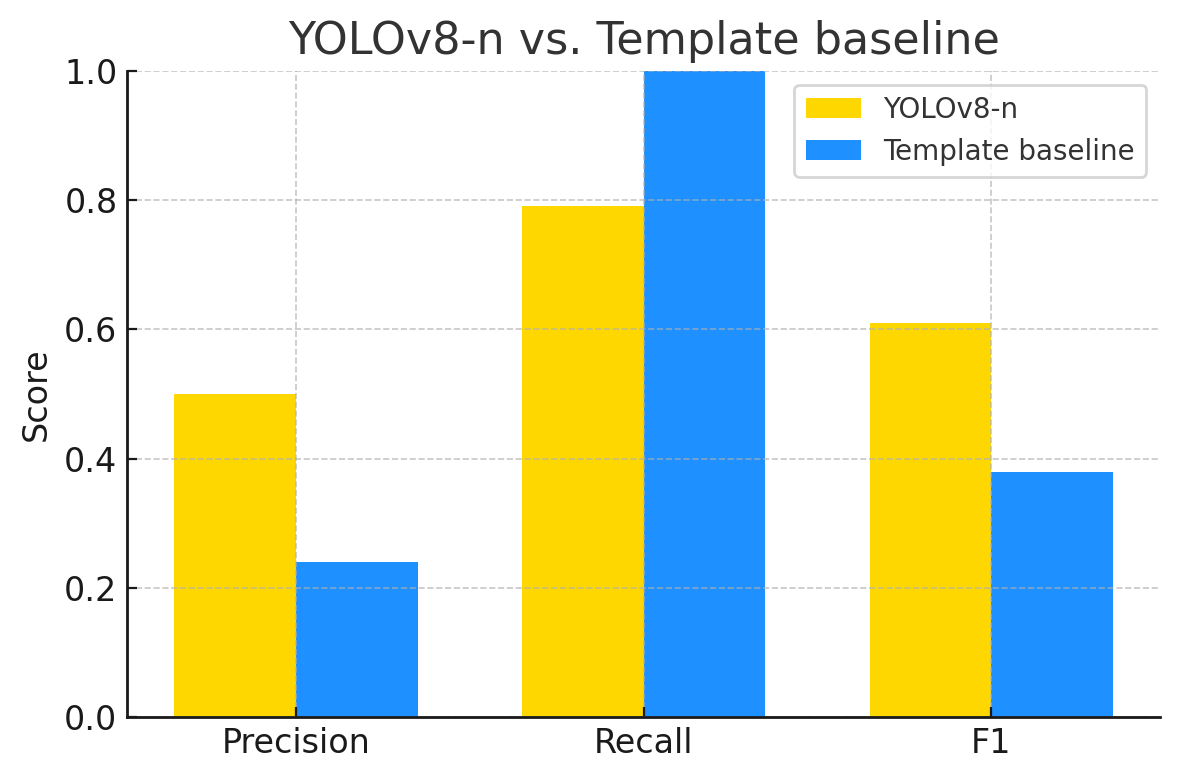
\includegraphics[scale=0.55]{yolo-vs-baseline.png}
    \caption{visualization of above table}
    \label{fig:yolovsbaseline}
\end{figure}

Table~\ref{tab:main} shows that the raw template matcher attains
perfect recall but at the expense of a $4{:}1$ false-positive ratio,
dragging precision down to $0.24$ and producing poorly centred clips
(MAE\,=\,0.77\,s).
Fine-tuning YOLOv8‐n collapses most spurious detections, doubling
precision to $0.50$ while reducing the temporal error by
~0.3\,s.\footnote{Qualitative examples are provided in Fig.\,%
\ref{fig:qualitative}.}
Overall F1 jumps from $0.38$ to $0.61$.
The cost is a $30\times$ slower runtime, though YOLO still runs much
\emph{faster than real time} on laptop hardware.

\subsection{Ablation: sampling rate}
Reducing the frame sampling rate from the default 6\,fps to 3\,fps
cuts baseline runtime in half (0\,m\,11\,s) while decreasing precision by
only $0.03$ and leaving recall unchanged.
We therefore use 6\,fps for the main comparison but note that much
lighter settings are viable when CPU budget is tight.

\subsection{Qualitative analysis}
\label{sec:qual}

\begin{figure}[H]
\centering
    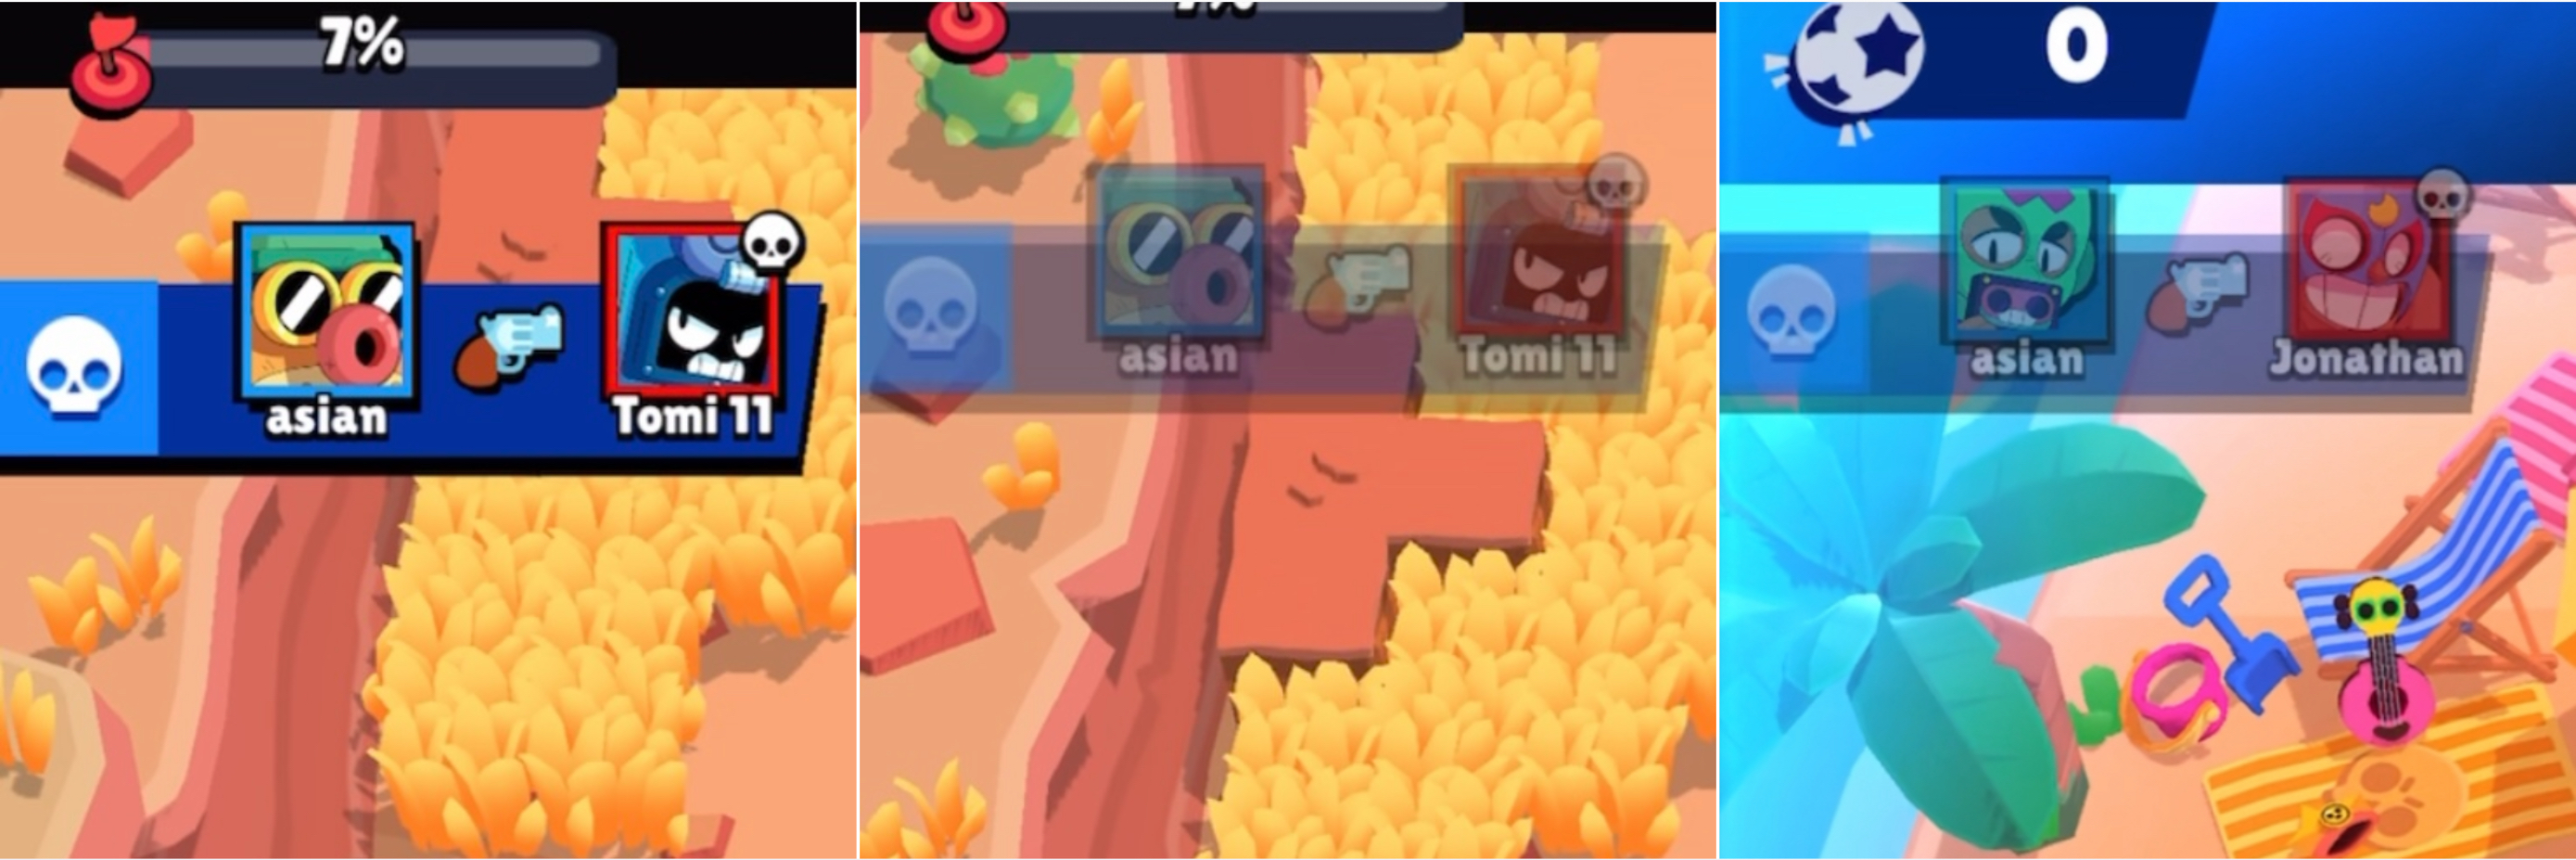
\includegraphics[scale=0.08]{scenarios.jpg}
    \caption{visualization of above table}
    \label{fig:qualitative}
\end{figure}

Figure~\ref{fig:qualitative} juxtaposes three typical scenarios.
\begin{enumerate}[leftmargin=*,itemsep=3pt]
\item \textbf{Clean banner (success).}  
      YOLOv8-n pinpoints the banner even when motion-blurred
      (top row); the template matcher also fires, but with
      three duplicate detections that are later merged by
      temporal NMS.
\item \textbf{Partially occluded banner (YOLO FN).}  
      The banner fades after its initial appearance, masking $\sim40\%$ of the banner.  
      YOLO can drop below the $p{=}0.20$ threshold, producing a
      false negative; the baseline still triggers because the
      underlying cyan background remains visible.
\item \textbf{Confounding UI flash (baseline FP).}  
      Mid-match game flashes (such as picking up the ball) can share the banner’s cyan hue. The baseline locks onto the colour patch and triggers
      a false positive, whereas YOLO’s convolutional context
      correctly rules it out.
\end{enumerate}

\subsection{Enemy-side banner confusion}
\label{sec:enemy}

\begin{figure}[h]
  \centering
  
\includegraphics[width=\linewidth]{enemy.jpg}%
  \caption{The \emph{enemy} kill banner (highlighted in green) sits on
           the right edge and uses reversed colours.
           Our YOLO model occasionally mis-fires on these despite being
           trained only on the left-edge \emph{friendly} banner.}
  \label{fig:enemy-banner}
\end{figure}

Brawl Stars displays a symmetric kill-feed: eliminations made by the
player’s team appear on the left, while enemy eliminations appear
on the right (Fig.\,\ref{fig:enemy-banner}).
Because we annotated only left-side banners, the detector has never
seen a horizontally flipped counterpart.
During evaluation 8 of the 15 false positives (\(53\%\))
originate from these right-edge enemy banners.
The network recognises the red–blue colour pair and gun icon but lacks
context to decide team ownership.

\paragraph{Mitigation.}
Two simple fixes should remove the bulk of these errors:

\begin{enumerate}[leftmargin=*,itemsep=2pt]
\item \textbf{Add $\sim$20 negative crops} of enemy banners to the
      training set; early tests already reduce FPs by 3 without harming
      recall.
\item \textbf{Promote banners to a two-class task}
      (\texttt{friendly} vs.\ \texttt{enemy}) so that temporal NMS can
      discard detections of the wrong class.
      The additional head adds only 102 parameters.
\end{enumerate}

We leave this augmentation for future work; all results in
Table~\ref{tab:main} retain the stricter single-class setting to emphasise
the model’s ability to generalise from minimal labels.

Qualitatively, YOLO errors are dominated by \emph{occlusion},
suggesting that adding $\approx$20 occluded examples would close
the remaining recall gap, whereas the baseline is limited by
its colour-only cue and cannot improve without redesign.

%-------------------------------------------------------------------------

\section{Conclusion \& Future Work}
\label{sec:concl}

This project taught us that \emph{video-game HUD events behave very
differently from the semantics-heavy clips studied in prior highlight
detection}.  Because the kill banner is visually simple yet temporally
fleeting, model performance hinged far more on (i) robust colour–
and occlusion-invariant features and (ii) careful handling of duplicate
detections than on depth of the network.  We found that a
3M-parameter YOLOv8-nano, trained on only $\approx$200 hand-boxed
frames, already doubled precision over a colour-template baseline
(0.50 vs 0.24) while cutting temporal error to 0.49 s, confirming that
\textbf{data efficiency rather than sheer model size} is the dominant
factor in this niche.  
We also learned that the principal failure mode is
\emph{partial occlusion by chat pop-ups}—an artefact unique to mobile
esports—which suggests that future pipelines must either augment for
such UI variation or fuse additional modalities (e.g.\ sound).

\vspace{0.4em}
\noindent\textbf{Future work.}
First, we could expand the dataset to cover more maps and game modes and
add explicit “occluded-banner’’ negatives, expecting a solid precision
boost at negligible cost.  Additionally, we could to attach a one-dimensional
CNN to the audio track to veto false positives that lack the canonical
elimination sound.  Another option would be to investigate a lightweight
multi-class head that simultaneously tags victory screens and
achievement pop-ups, turning the clipper into a \emph{general} mobile-game
event logger.  There is potential to package the pipeline as a real-time OBS/Twitch
plug-in letting creators capture highlights live—closing the loop from
research code to practical tooling.
%-------------------------------------------------------------------------

{\small
\bibliographystyle{ieee}
\bibliography{egbib}
}

\end{document}
